\section{Sensor-level comparisons for period means}
\label{sec:annual_mean_comparison}
In this section, we analyze whether period means vary on a sensor basis. Given that the period and daily means seldom exhibit spatial autocorrelation in the two original full-year networks, we aim to understand whether the sensor period means themselves may be considered as samples from the same underlying distribution, or for each sensor $i$, $\hat{\mu}_i = \mu_{\text{reference}}$. If this were not the case for a majority of the sensors, then it would make sense to control for that sensor-specific mean when analyzing spatial autocorrelation. In the context of air pollution, this result would further support the hypothesis that there are sensors which are consistently exposed to higher (or lower) levels of \pmtt\ than other sensors in the network.

A simple technique to test this hypothesis would be to perform a one-way ANOVA, but this procedure crucially assumes independence. Because each sensor's mean is comprised of a set of temporally auto-correlated observations, the variance would be underestimated under such a procedure (and indeed, when we performed this test, the resulting $p$-value was $<<1\times10^{-10}$). We account for temporal auto-correlation by using a gap-aware generalized least squares (GLS) estimate of the mean, assuming an AR(1) structured error term and treating each sensor as independent. As discussed in Section~\ref{sec:si_gls}, the result of this correlation is a reduced effective sample size (i.e., a larger variance for the estimator $\hat{\mu}_i$), and consequently, a wider confidence interval for the mean. Furthermore, to compare the family-wise adherence to the same mean (i.e., the multiple comparisons problem), we adjust the $\alpha=0.05$ critical value (used for a 95\% confidence interval) with a Bonferroni correction. For $K$ sensors in the network, this correction alters the $z$-score used for standard confidence intervals by substituting $\alpha_{B}=\alpha/K$. The resulting confidence interval is then $(\hat{\mu}_i \pm z_{1-\alpha_B/2}\sqrt{\text{Var}(\hat{\mu}_i)})$.

We visualize these confidence intervals against the reference mean in Figure~\ref{fig:mult_comparisons_plots}. In the full-year networks, 2 \city{Dhaka} sensors and 4 \city{Lucknow} sensors have adjusted 95\% confidence intervals which do not contain the reference mean. Without the Bonferroni correction, this number becomes 5 in each city. These results support the conclusion that mean behavior is largely homogeneous across sensors. Intuitively, this statement aligns with our expectations: because the majority of air pollution variability is dominated by regional and seasonal phenomena, we expect that the means should not have significant variance across sensors. In the cases where the sensors do deviate significantly from the reference mean, there were significant missing data during the most polluted portions of the year (December through February). As a result, the computed mean and variance estimates are lower than would be expected.

For \city{Chicago}, the comparable check is treated as a partial-year descriptive screen rather than a full annual ANOVA analogue. Applying the same gap-aware AR(1) GLS logic to the official-daily calibrated data gives 12/277 sensors whose Bonferroni-adjusted confidence intervals exclude the network reference mean, with a median daily presence of 99.6\% and a median GLS effective sample size of 78.8 days. This proportion remains small (4.3\%) despite the much larger Chicago network and stricter Bonferroni threshold ($\alpha_B = 0.05/277$), supporting the same qualitative conclusion that the network is dominated by a shared temporal signal. We do not interpret this as a full-year Chicago stationarity test because the available window spans September--May rather than a complete seasonal cycle.

\begin{figure}[H]
 \centering
 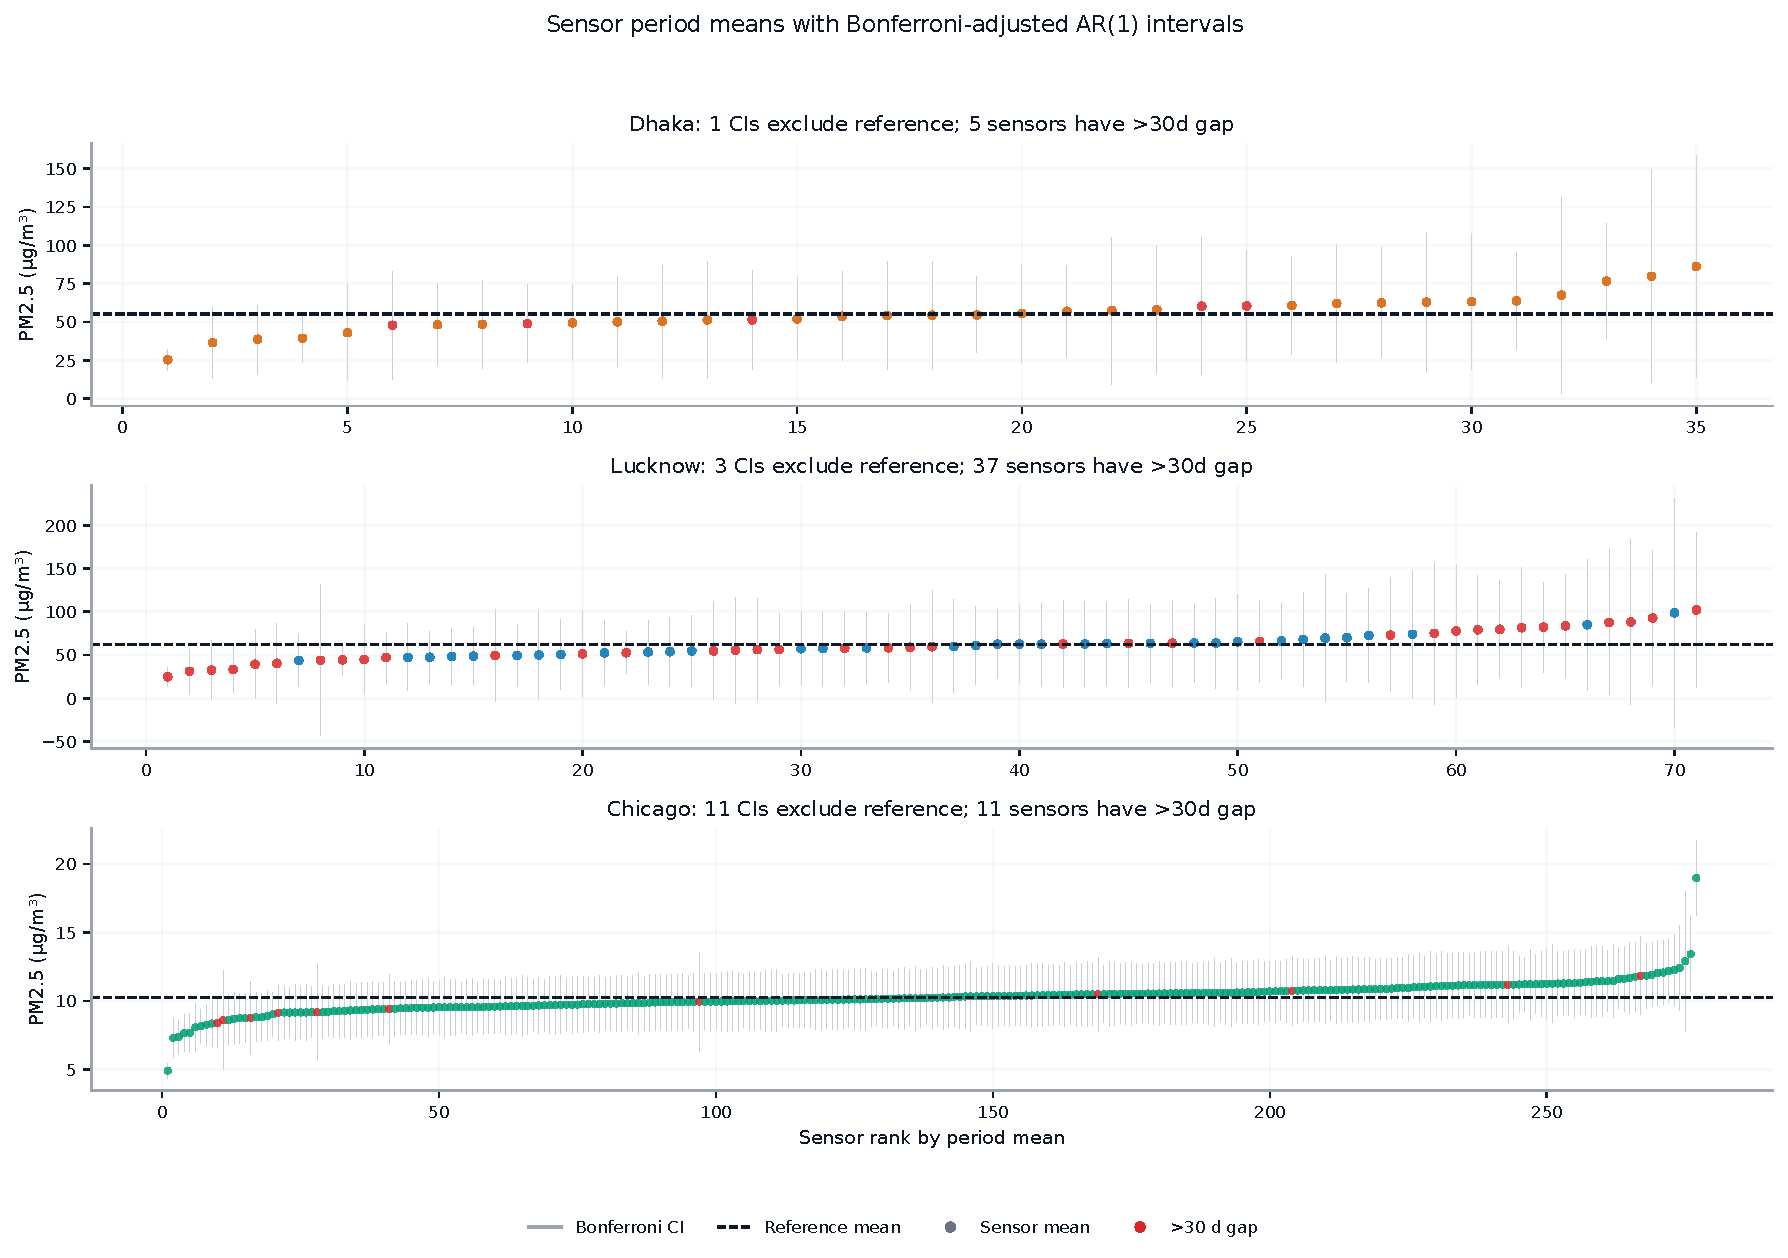
\includegraphics[width=0.95\textwidth]{Plots/Supporting_Information/Figure_SI_11/three_city_period_sensor_means_bonferroni_ci.pdf}
 \caption{Per-sensor period mean estimates with 95\% Bonferroni-adjusted confidence intervals for \city{Dhaka}, \city{Lucknow}, and \city{Chicago}. The dashed line in each panel marks the reference-network mean. In \city{Dhaka} and \city{Lucknow}, 2 of 35 and 4 of 71 sensor intervals respectively fall outside the reference mean; in \city{Chicago}, 12 of 277 do, a comparably small proportion (4.3\%) given the much stricter Bonferroni threshold. The \city{Chicago} panel covers the nine-month deployment window.}
 \label{fig:mult_comparisons_plots}
\end{figure}
